\documentclass[../main.tex]{subfiles}
\graphicspath{{\subfix{../images/}}}
\begin{document}


\begin{figure}[htb!]
  \centering
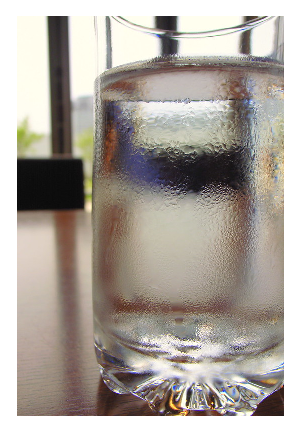
\includegraphics[width=5cm]{GlassWater.eps}
  \caption{A glass of water~\cite{GlassWater}}
\end{figure}



Water doesn't contain any nutrients, but nevertheless is water of the biggest importance for the human body.
Without water, there's no life.
The human body consists our of about 60\% water (a newborn even up to 75\%).
Roughly 60\% of that water is found in the intracellular space (inside the cells).
The rest is in between the cells in the form of interstitial fluids (between the cells),
like blood plasma, lymph, urine, saliva, digestion fluids, tear liquid, nose secretes and sweat.


In the human organism, water mainly serves:
\begin{itemize}
\item to cover the needs of fluids in cells and tissues,
\item as a solvent and medium of transportation for nutrients, enzymes, hormones and so on,
\item to excrete metabolism end products over the urine,
\item to regulate the body temperature.
\end{itemize}

\subsection{How much Water does a Human Being Need?}

During a day, the human body looses\index{water consumption} \SIrange{2}{2.5}{\liter}
(\SIrange[parse-numbers=false]{\text{\ensuremath{8\sfrac{1}{2}}}}{\text{\ensuremath{10\sfrac{1}{2}}}}{\cup}) of water, of which:
\begin{itemize}
\item \SIrange{1.0}{1.5}{\L}
  %(4\sfrac{1}{4}\ -- 6\sfrac{1}{4}\ cups)
  (\SIrange[parse-numbers=false]{\text{\ensuremath{4\sfrac{1}{4}}}}{\text{\ensuremath{6\sfrac{1}{4}}}}{\cup}) through the urine
\item \SIrange{0.4}{1.0}{\L}
  %(1\sfrac{3}{4}\ -- 4\sfrac{1}{4}\ cups)
  (\SIrange[parse-numbers=false]{\text{\ensuremath{1\sfrac{3}{4}}}}{\text{\ensuremath{4\sfrac{1}{4}}}}{\cup}) through respiration
\item \SIrange{0.1}{0.5}{\L}
  %(3\sfrac{1}{2}\ fl.oz. -- 2\sfrac{1}{8}\ cups)
  (\SIrange[parse-numbers=false]{\text{\ensuremath{3\sfrac{1}{2}}}}{\text{\ensuremath{2\sfrac{1}{8}}}}{\cup}) over the skin, through sweat
\item \SIrange{0.1}{0.2}{\L}
  %(3\sfrac{1}{2}\ -- 7 fl.oz.)
  (\SIrange[parse-numbers=false]{\text{\ensuremath{3\sfrac{1}{2}}}}{\text{\ensuremath{7}}}{\cup}) through feces
  \end{itemize}

  This loss of water has to be added back to our body on a daily base, through drinking and eating.
  For a healthy, barely physical active person, that means a daily fluid intake of about \SIrange{30}{35}{\mL} of fluids per \unit{\kg}
  (\SIrange{0.45}{0.54}{\floz/\lbs}) body weight.
  A person who weights \SI{70}{\kg} (\SI{154}{\lbs}) therefore needs a fluid supply of
  \SIrange{2.0}{2.5}{\L}
  %(8\sfrac{1}{2}\ -- 10\sfrac{1}{2} cups)
  (\SIrange[parse-numbers=false]{\text{\ensuremath{8\sfrac{1}{2}}}}{\text{\ensuremath{10\sfrac{1}{2}}}}{\cup}) per day.
  Out of this amount, about \SIrange{0.5}{1}{\L}
  %(2\sfrac{1}{8}\ -- 4\sfrac{1}{4} cups)
  (\SIrange[parse-numbers=false]{\text{\ensuremath{2\sfrac{1}{8}}}}{\text{\ensuremath{4\sfrac{1}{4}}}}{\cup})
  fluids will be supplied through food (veggies, fruits, \ldots).
  This results then in the recommended amount of drinking about \SIrange{1}{2}{\L} (\SIrange{1}{2}{\quart}) of fluids a day.

  Please consider, that the water usage also depends on the outside temperature, physical activity levels and the state of health.
  When it's hot, under heavy physical labor or sport, sweating will cool down the body and
  in case of disease (fever, diarrhea, vomiting) the body will also loose a lot of additional water.
  All these losses need to be compensated with additional fluid intake.

  \subsection{Is Water the Best Drink?}

  As drinks counts foods, which pretty much only furnish water to our body. 
  Fruit and veggie juices, milk, yogurt drinks and soft drinks deliver next to water plenty of nutrients and energy and  don't really count as drinks.
  Alcoholic drinks are non--essential food items, stimulants and are very bad at hydrating our body.
  On top of that, they are delivering a lot of unwanted energy (about \SI{7}{\kcal/\g}, roughly \SI{200}{\kcal/\oz}).

% Swiss tap water - US tap water?
  
  Pure water is by far the best and cheapest drink. Tap water, depending on location filtered, is the best option to hydrate.
  In order to change things up, can water be flavored in different ways:
  \begin{itemize}
  \item Fruit or herbal tea
  \item Black or green tea* 
  \item Broth
  \item Coffee*
    \item Lemon water (juice of one lemon for one Liter (quart) of water)
  \end{itemize}
{\footnotesize{*See special drinks and foods in the section \ref{SpecialFoods}, page~\pageref{SpecialFoods}.}}
  
People who are depended on bottled water, should preferably choose still water.
  The carbonation leeches vital oxygen from our body and adds unnecessary acids to our system.

  \subsection[Drinking Too Little, Too Much or the Wrong Drinks]{People Who Drink Not Enough, Too Much or the Wrong Things Risk their Health}

  Humans can survive multiple weeks without food, but without fluids only three days.
  Already a loss of fluids of 1\% or our body weight leads to the first symptoms like head ache, difficulties focusing and thirst.
  Being thirsty already indicates a lack in fluids.
  With advances age, the thirst signal decreases, which in turn is the reason that older people often don't drink enough.
  Among other effects, this leads to:
  \begin{itemize}
  \item higher viscosity of the blood, with the danger of thrombosis and a decreased oxygen supply of the organs
  \item dry skin, which is easier to be hurt
  \item drier mucous membranes, which are more susceptible to infections
    \item constipation, through excessive thickening of the feces
    \end{itemize}

    An excessive intake in fluids also can threaten the physical productivity and in excess even get dangerous.
    But the biggest danger comes from the many calories, if soft drinks or alcoholic drinks get consumed in excess. 

 
\vspace{5mm}
\noindent
\begin{fminipage}{\textwidth}
  \textbf{Profile Water}
  \begin{itemize}
  \item The human body consists of 60\% of water and a human can only survive three days without water intake
  \item Water is vital for humans, it transports nutrients, enzymes and hormones to the cells; it helps the excretion of harmful substances and the regulation of the body temperature
  \item Water is free of calories and doesn't deliver energy to the body
  \item We need about \SIrange{2}{2.5}{\L}
    %(8\sfrac{1}{2}\ -- 10\sfrac{1}{2}\ cups)
    (\SIrange[parse-numbers=false]{\text{\ensuremath{8\sfrac{1}{2}}}}{\text{\ensuremath{10\sfrac{1}{2}}}}{\cup}) of fluids a day, thereof
    \SIrange{1}{2}{\L}
    (\SIrange{1}{2}{\quart}) in the form of water
    \item Preferably pure water or mineral water without carbonation
  \end{itemize}
\end{fminipage}


\end{document}
